% Options for packages loaded elsewhere
% Options for packages loaded elsewhere
\PassOptionsToPackage{unicode}{hyperref}
\PassOptionsToPackage{hyphens}{url}
%
\documentclass[
  11pt,
  ignorenonframetext,
  aspectratio=169,
]{beamer}
\newif\ifbibliography
\usepackage{pgfpages}
\setbeamertemplate{caption}[numbered]
\setbeamertemplate{caption label separator}{: }
\setbeamercolor{caption name}{fg=normal text.fg}
\beamertemplatenavigationsymbolsempty
% remove section numbering
\setbeamertemplate{part page}{
  \centering
  \begin{beamercolorbox}[sep=16pt,center]{part title}
    \usebeamerfont{part title}\insertpart\par
  \end{beamercolorbox}
}
\setbeamertemplate{section page}{
  \centering
  \begin{beamercolorbox}[sep=12pt,center]{section title}
    \usebeamerfont{section title}\insertsection\par
  \end{beamercolorbox}
}
\setbeamertemplate{subsection page}{
  \centering
  \begin{beamercolorbox}[sep=8pt,center]{subsection title}
    \usebeamerfont{subsection title}\insertsubsection\par
  \end{beamercolorbox}
}
% Prevent slide breaks in the middle of a paragraph
\widowpenalties 1 10000
\raggedbottom
\AtBeginPart{
  \frame{\partpage}
}
\AtBeginSection{
  \ifbibliography
  \else
    \frame{\sectionpage}
  \fi
}
\AtBeginSubsection{
  \frame{\subsectionpage}
}
\usepackage{iftex}
\ifPDFTeX
  \usepackage[T1]{fontenc}
  \usepackage[utf8]{inputenc}
  \usepackage{textcomp} % provide euro and other symbols
\else % if luatex or xetex
  \usepackage{unicode-math} % this also loads fontspec
  \defaultfontfeatures{Scale=MatchLowercase}
  \defaultfontfeatures[\rmfamily]{Ligatures=TeX,Scale=1}
\fi
\usepackage{lmodern}

\ifPDFTeX\else
  % xetex/luatex font selection
\fi
% Use upquote if available, for straight quotes in verbatim environments
\IfFileExists{upquote.sty}{\usepackage{upquote}}{}
\IfFileExists{microtype.sty}{% use microtype if available
  \usepackage[]{microtype}
  \UseMicrotypeSet[protrusion]{basicmath} % disable protrusion for tt fonts
}{}
\makeatletter
\@ifundefined{KOMAClassName}{% if non-KOMA class
  \IfFileExists{parskip.sty}{%
    \usepackage{parskip}
  }{% else
    \setlength{\parindent}{0pt}
    \setlength{\parskip}{6pt plus 2pt minus 1pt}}
}{% if KOMA class
  \KOMAoptions{parskip=half}}
\makeatother

\usepackage{color}
\usepackage{fancyvrb}
\newcommand{\VerbBar}{|}
\newcommand{\VERB}{\Verb[commandchars=\\\{\}]}
\DefineVerbatimEnvironment{Highlighting}{Verbatim}{commandchars=\\\{\}}
% Add ',fontsize=\small' for more characters per line
\usepackage{framed}
\definecolor{shadecolor}{RGB}{241,243,245}
\newenvironment{Shaded}{\begin{snugshade}}{\end{snugshade}}
\newcommand{\AlertTok}[1]{\textcolor[rgb]{0.68,0.00,0.00}{#1}}
\newcommand{\AnnotationTok}[1]{\textcolor[rgb]{0.37,0.37,0.37}{#1}}
\newcommand{\AttributeTok}[1]{\textcolor[rgb]{0.40,0.45,0.13}{#1}}
\newcommand{\BaseNTok}[1]{\textcolor[rgb]{0.68,0.00,0.00}{#1}}
\newcommand{\BuiltInTok}[1]{\textcolor[rgb]{0.00,0.23,0.31}{#1}}
\newcommand{\CharTok}[1]{\textcolor[rgb]{0.13,0.47,0.30}{#1}}
\newcommand{\CommentTok}[1]{\textcolor[rgb]{0.37,0.37,0.37}{#1}}
\newcommand{\CommentVarTok}[1]{\textcolor[rgb]{0.37,0.37,0.37}{\textit{#1}}}
\newcommand{\ConstantTok}[1]{\textcolor[rgb]{0.56,0.35,0.01}{#1}}
\newcommand{\ControlFlowTok}[1]{\textcolor[rgb]{0.00,0.23,0.31}{\textbf{#1}}}
\newcommand{\DataTypeTok}[1]{\textcolor[rgb]{0.68,0.00,0.00}{#1}}
\newcommand{\DecValTok}[1]{\textcolor[rgb]{0.68,0.00,0.00}{#1}}
\newcommand{\DocumentationTok}[1]{\textcolor[rgb]{0.37,0.37,0.37}{\textit{#1}}}
\newcommand{\ErrorTok}[1]{\textcolor[rgb]{0.68,0.00,0.00}{#1}}
\newcommand{\ExtensionTok}[1]{\textcolor[rgb]{0.00,0.23,0.31}{#1}}
\newcommand{\FloatTok}[1]{\textcolor[rgb]{0.68,0.00,0.00}{#1}}
\newcommand{\FunctionTok}[1]{\textcolor[rgb]{0.28,0.35,0.67}{#1}}
\newcommand{\ImportTok}[1]{\textcolor[rgb]{0.00,0.46,0.62}{#1}}
\newcommand{\InformationTok}[1]{\textcolor[rgb]{0.37,0.37,0.37}{#1}}
\newcommand{\KeywordTok}[1]{\textcolor[rgb]{0.00,0.23,0.31}{\textbf{#1}}}
\newcommand{\NormalTok}[1]{\textcolor[rgb]{0.00,0.23,0.31}{#1}}
\newcommand{\OperatorTok}[1]{\textcolor[rgb]{0.37,0.37,0.37}{#1}}
\newcommand{\OtherTok}[1]{\textcolor[rgb]{0.00,0.23,0.31}{#1}}
\newcommand{\PreprocessorTok}[1]{\textcolor[rgb]{0.68,0.00,0.00}{#1}}
\newcommand{\RegionMarkerTok}[1]{\textcolor[rgb]{0.00,0.23,0.31}{#1}}
\newcommand{\SpecialCharTok}[1]{\textcolor[rgb]{0.37,0.37,0.37}{#1}}
\newcommand{\SpecialStringTok}[1]{\textcolor[rgb]{0.13,0.47,0.30}{#1}}
\newcommand{\StringTok}[1]{\textcolor[rgb]{0.13,0.47,0.30}{#1}}
\newcommand{\VariableTok}[1]{\textcolor[rgb]{0.07,0.07,0.07}{#1}}
\newcommand{\VerbatimStringTok}[1]{\textcolor[rgb]{0.13,0.47,0.30}{#1}}
\newcommand{\WarningTok}[1]{\textcolor[rgb]{0.37,0.37,0.37}{\textit{#1}}}

\usepackage{longtable,booktabs,array}
\newcounter{none} % for unnumbered tables
\usepackage{calc} % for calculating minipage widths
\usepackage{caption}
% Make caption package work with longtable
\makeatletter
\def\fnum@table{\tablename~\thetable}
\makeatother
\usepackage{graphicx}
\makeatletter
\newsavebox\pandoc@box
\newcommand*\pandocbounded[1]{% scales image to fit in text height/width
  \sbox\pandoc@box{#1}%
  \Gscale@div\@tempa{\textheight}{\dimexpr\ht\pandoc@box+\dp\pandoc@box\relax}%
  \Gscale@div\@tempb{\linewidth}{\wd\pandoc@box}%
  \ifdim\@tempb\p@<\@tempa\p@\let\@tempa\@tempb\fi% select the smaller of both
  \ifdim\@tempa\p@<\p@\scalebox{\@tempa}{\usebox\pandoc@box}%
  \else\usebox{\pandoc@box}%
  \fi%
}
% Set default figure placement to htbp
\def\fps@figure{htbp}
\makeatother





\setlength{\emergencystretch}{3em} % prevent overfull lines

\providecommand{\tightlist}{%
  \setlength{\itemsep}{0pt}\setlength{\parskip}{0pt}}



 


\setbeamertemplate{navigation symbols}{}
\setbeamertemplate{footline}[frame number]
\setbeamertemplate{itemize items}[circle]
\setbeamertemplate{itemize subitem}[triangle]
\setbeamercolor{frametitle}{fg=black}
\setbeamerfont{frametitle}{series=\bfseries}
\newcommand{\indep}{\perp\!\!\!\perp}
\usepackage{amsmath}
\usepackage{setspace}
\DeclareMathOperator*{\argmin}{arg\,min}
\usepackage{booktabs}
\usepackage{array}
\newcolumntype{R}[1]{>{\raggedright\arraybackslash}p{#1}}
\usepackage{tikz}
\usetikzlibrary{arrows.meta,positioning,calc}
\tikzset{
  dnode/.style={circle,draw,thick,minimum size=9mm,inner sep=1pt,font=\small},
  unode/.style={circle,draw,thick,dashed,minimum size=9mm,inner sep=1pt,font=\small},
  qnode/.style={circle,draw,thick,dotted,minimum size=9mm,inner sep=1pt,font=\small},
  de/.style={-{Stealth[length=2.2mm]},thick},
  dde/.style={-{Stealth[length=2.2mm]},thick,dashed}
}
\usepackage{fancyvrb}
\fvset{fontsize=\scriptsize}
\makeatletter
\def\verbatim@font{\scriptsize\ttfamily}
\makeatother
\makeatletter
\@ifpackageloaded{caption}{}{\usepackage{caption}}
\AtBeginDocument{%
\ifdefined\contentsname
  \renewcommand*\contentsname{Table of contents}
\else
  \newcommand\contentsname{Table of contents}
\fi
\ifdefined\listfigurename
  \renewcommand*\listfigurename{List of Figures}
\else
  \newcommand\listfigurename{List of Figures}
\fi
\ifdefined\listtablename
  \renewcommand*\listtablename{List of Tables}
\else
  \newcommand\listtablename{List of Tables}
\fi
\ifdefined\figurename
  \renewcommand*\figurename{Figure}
\else
  \newcommand\figurename{Figure}
\fi
\ifdefined\tablename
  \renewcommand*\tablename{Table}
\else
  \newcommand\tablename{Table}
\fi
}
\@ifpackageloaded{float}{}{\usepackage{float}}
\floatstyle{ruled}
\@ifundefined{c@chapter}{\newfloat{codelisting}{h}{lop}}{\newfloat{codelisting}{h}{lop}[chapter]}
\floatname{codelisting}{Listing}
\newcommand*\listoflistings{\listof{codelisting}{List of Listings}}
\makeatother
\makeatletter
\makeatother
\makeatletter
\@ifpackageloaded{caption}{}{\usepackage{caption}}
\@ifpackageloaded{subcaption}{}{\usepackage{subcaption}}
\makeatother

\usepackage{bookmark}
\IfFileExists{xurl.sty}{\usepackage{xurl}}{} % add URL line breaks if available
\urlstyle{same}
\hypersetup{
  pdftitle={Causal Panel Designs},
  pdfauthor={Professor Ji-Woong Chung},
  hidelinks,
  pdfcreator={LaTeX via pandoc}}


\title{\texorpdfstring{Causal Panel Designs}{Causal Panel Designs}}
\subtitle{\texorpdfstring{BUSS975: Causal Inference in Financial
Research}{BUSS975: Causal Inference in Financial Research}}
\author{Professor Ji-Woong Chung}
\date{}
\institute{Korea University}

\begin{document}
\frame{\titlepage}


\begin{frame}{Where we left off}
\protect\phantomsection\label{where-we-left-off}
\begin{itemize}
\tightlist
\item
  Lecture 5 spent its time looking for a \textbf{shock}: a lottery, a
  judge, a national surge, a threshold, the weather. Something that
  moved treatment for reasons the unit did not choose.
\item
  Good instruments are scarce. Most of the time you do not have one.
\end{itemize}

\vspace{0.4em}

\begin{itemize}
\tightlist
\item
  Panel data offers a different trade. Instead of finding a shock,
  \textbf{use the unit as its own control}.
\item
  If you see the same firm in \(2015\) and in \(2019\), anything about
  that firm which did not change in between cannot explain why its
  outcome changed.
\end{itemize}
\end{frame}

\begin{frame}{The plan}
\protect\phantomsection\label{the-plan}
\begin{enumerate}
\tightlist
\item
  \textbf{What panel data is} --- and what the structure buys you.
\item
  \textbf{Pooled OLS}, and the two separate ways it fails.
\item
  \textbf{Fixed effects}, the \emph{within} estimator: the
  transformation, three ways to compute it, the assumptions.
\item
  \textbf{Three estimators side by side}, on data where we know the
  right answer.
\item
  \textbf{Inference}: clustering, and what to do when clusters are few.
\item
  \textbf{What fixed effects cannot fix} --- two identification
  failures, then four costs.
\item
  \textbf{Fixed effects in finance}: richer effects, and the comparison
  each one leaves.
\end{enumerate}
\end{frame}

\section{1. What Panel Data Is}\label{what-panel-data-is}

\begin{frame}{Two things that get called the same name}
\protect\phantomsection\label{two-things-that-get-called-the-same-name}
\begin{center}\small
\begin{tabular}{lll}
\toprule
 & You follow & Example \\
\midrule
\textbf{Panel} (longitudinal) & the \emph{same} units over time & Compustat firm-years \\
\textbf{Repeated cross-section} & a fresh sample each period & the Census, most surveys \\
\bottomrule
\end{tabular}
\end{center}

\begin{itemize}
\tightlist
\item
  Only a true panel lets you difference a unit against \textbf{itself}.
  A repeated cross-section lets you difference \emph{groups} against
  themselves, which is a weaker but still useful thing.
\item
  Notation throughout: \(i = 1, \dots, N\) units, \(t = 1, \dots, T\)
  periods. We assume a \textbf{balanced} panel, so every unit appears in
  every period.
\end{itemize}
\end{frame}

\begin{frame}{Motivation: a regression you have all run}
\protect\phantomsection\label{motivation-a-regression-you-have-all-run}
\[
\text{leverage}_{i,j,t} \;=\; \beta_0 + \beta_1 \text{profitability}_{i,j,t} + u_{i,j,t}
\]

for firm \(i\) in industry \(j\) in year \(t\). \textbf{What is in
\(u\)?}

\vspace{0.3em}

\begin{itemize}
\tightlist
\item
  Managerial talent and managerial risk aversion. Industry supply and
  demand shocks. The firm's cost of capital and its investment
  opportunity set. Local institutions and financial development.
\end{itemize}

\vspace{0.3em}

\begin{itemize}
\tightlist
\item
  Every one of these plausibly moves leverage \textbf{and} correlates
  with profitability.
\item
  \textbf{Why not just use a proxy?} A proxy delivers consistency only
  if the unobservable is uncorrelated with the regressors \emph{after}
  conditioning on it. That is a demanding requirement, and you cannot
  check it.
\end{itemize}
\end{frame}

\begin{frame}{The confounding, as a picture}
\protect\phantomsection\label{the-confounding-as-a-picture}
\begin{center}
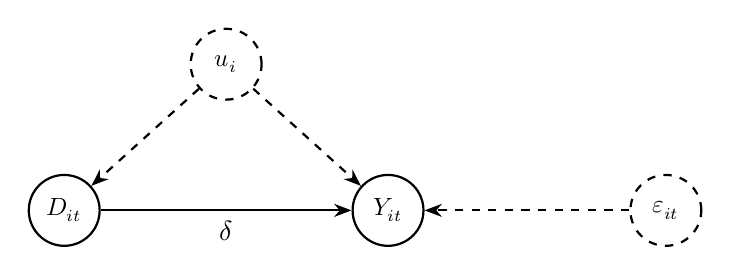
\begin{tikzpicture}[node distance=14mm]
  \node[unode] (u) {$u_i$};
  \node[dnode, below left=12mm and 14mm of u] (d) {$D_{it}$};
  \node[dnode, below right=12mm and 14mm of u] (y) {$Y_{it}$};
  \node[unode, right=26mm of y] (e) {$\varepsilon_{it}$};
  \draw[dde] (u) -- (d);
  \draw[dde] (u) -- (y);
  \draw[de]  (d) -- node[below]{$\delta$} (y);
  \draw[dde] (e) -- (y);
\end{tikzpicture}
\end{center}

\vspace{-0.3em}

\begin{itemize}
\tightlist
\item
  \(u_i\) is a \textbf{confounder}: it causes the treatment and it
  causes the outcome.
\item
  Ordinarily that would be the end of the story --- you cannot condition
  on what you cannot see.
\item
  \textbf{But \(u_i\) carries no \(t\) subscript.} It is the same number
  in every period for a given unit.
\end{itemize}
\end{frame}

\begin{frame}{The model}
\protect\phantomsection\label{the-model}
For each unit \(i\) in period \(t\):

\[
Y_{it} \;=\; \alpha + \delta D_{it} \;+\; \underbrace{u_i}_{\substack{\text{unobserved} \\ \text{heterogeneity}}} \;+\; \underbrace{\varepsilon_{it}}_{\substack{\text{idiosyncratic} \\ \text{error}}}, \qquad t = 1, \dots, T .
\]

Reading it with the schooling--earnings example:

\begin{center}\small
\begin{tabular}{ll}
\toprule
$Y_{it}$ & log earnings of person $i$ in year $t$ \\
$D_{it}$ & schooling --- the treatment, and it must \textbf{change} over time \\
$\delta$ & the returns to schooling --- assumed the \emph{same} for everyone \\
$u_i$ & everything about $i$ that never changes: ability, upbringing, drive \\
$\varepsilon_{it}$ & everything that changes period to period: luck, health, the cycle \\
\bottomrule
\end{tabular}
\end{center}
\end{frame}

\section{2. Pooled OLS}\label{pooled-ols}

\begin{frame}{Ignoring the panel structure}
\protect\phantomsection\label{ignoring-the-panel-structure}
Throw the time dimension away and regress \(Y_{it}\) on \(D_{it}\):

\[
Y_{it} = \alpha + \delta D_{it} + \eta_{it}, \qquad \eta_{it} \equiv u_i + \varepsilon_{it} .
\]

\begin{itemize}
\tightlist
\item
  This is \textbf{pooled OLS (POLS)}.
\item
  POLS needs only \textbf{contemporaneous exogeneity}: the error is
  unrelated to treatment \emph{in the same period}, \[
  E[\eta_{it} \mid D_{it}] = 0, \qquad t = 1, \dots, T .
  \]
\item
  But \(u_i\) sits inside \(\eta_{it}\), so this requires \(u_i\) to be
  \textbf{uncorrelated with treatment} --- exactly what the picture
  denies.
\end{itemize}
\end{frame}

\begin{frame}{POLS fails twice, not once}
\protect\phantomsection\label{pols-fails-twice-not-once}
\begin{itemize}
\tightlist
\item
  \textbf{Failure 1: bias.} \(u_i\) is in the error and correlated with
  \(D_{it}\). \(\Rightarrow\) Omitted variable bias.
\end{itemize}

\vspace{0.4em}

\begin{itemize}
\tightlist
\item
  \textbf{Failure 2: the standard errors.} \(u_i\) appears in
  \(\eta_{it}\) for \textbf{every} period of unit \(i\). So the errors
  of the same unit are correlated with each other by construction ---
  serial correlation.

  \begin{itemize}
  \tightlist
  \item
    The reported standard errors are therefore \textbf{too small}, often
    by a lot. You get a tight interval around a biased number.
  \end{itemize}
\end{itemize}
\end{frame}

\section{3. Fixed Effects: The Within
Estimator}\label{fixed-effects-the-within-estimator}

\begin{frame}{The idea in one line}
\protect\phantomsection\label{the-idea-in-one-line}
\begin{quote}
Stop comparing person \(i\) to person \(j\). Compare person \(i\) to
\textbf{person \(i\) at another date}.
\end{quote}

\vspace{0.5em}

\begin{itemize}
\tightlist
\item
  Any confounder that is the same in both of \(i\)'s periods cannot
  explain a change between them.
\item
  This works \textbf{whether or not you can observe the confounder}, and
  whether or not you can name it.
\item
  The price is equally sharp: the only variation left is variation
  \textbf{within} units. Units that never change contribute nothing.
\item
  So the estimate is built entirely from \textbf{switchers} --- people
  whose schooling changed, firms whose policy changed. Name them before
  you interpret the number.
\end{itemize}
\end{frame}

\begin{frame}{Where did \(u_i\) go?}
\protect\phantomsection\label{where-did-u_i-go}
Average the model over time for a single unit \(i\): \[
\bar Y_i = \alpha + \delta \bar D_i + u_i + \bar\varepsilon_i,
\qquad \text{where } \bar Y_i = \tfrac{1}{T}\textstyle\sum_t Y_{it} .
\] Now subtract that from the original equation, period by period: \[
\underbrace{(Y_{it} - \bar Y_i)}_{\ddot Y_{it}}
= \delta \underbrace{(D_{it} - \bar D_i)}_{\ddot D_{it}}
+ \underbrace{(\alpha - \alpha)}_{\textstyle = \;0}
+ \underbrace{(u_i - u_i)}_{\textstyle = \;0}
+ \underbrace{(\varepsilon_{it} - \bar\varepsilon_i)}_{\ddot\varepsilon_{it}} .
\] \vspace{-0.2em} \[
\boxed{\;\ddot Y_{it} = \delta \ddot D_{it} + \ddot\varepsilon_{it}\;}
\]

\begin{itemize}
\tightlist
\item
  The price: \(\ddot\varepsilon_{it}\) contains \(\bar\varepsilon_i\),
  which averages \textbf{every} period's shock. So \(D_{it}\) must be
  unrelated to the shocks of \emph{all} periods, not just its own ---
  \textbf{strict exogeneity}.
\end{itemize}
\end{frame}

\begin{frame}{The same thing, as a minimisation problem}
\protect\phantomsection\label{the-same-thing-as-a-minimisation-problem}
Treat the \(u_i\) as \(N\) parameters to be estimated alongside
\(\delta\): \[
(\hat\delta,\, \hat u_1, \dots, \hat u_N) \;=\; \argmin_{b,\, m_1, \dots, m_N} \; \sum_{i=1}^{N} \sum_{t=1}^{T} \big(Y_{it} - D_{it} b - m_i\big)^2 .
\]

\begin{itemize}
\item
  This is a regression of \(Y_{it}\) on \(D_{it}\) \textbf{plus \(N\)
  individual dummies}.
\item
  The first-order condition with respect to \(m_i\) gives, for each
  unit, \[
  \hat m_i \;=\; \frac{1}{T}\sum_{t=1}^{T}\big(Y_{it} - D_{it}\hat\delta\big) \;=\; \bar Y_i - \bar D_i \hat\delta .
  \]
\item
  The estimated fixed effect \(\hat m_i\) is simply unit \(i\)'s average
  residual.
\end{itemize}
\end{frame}

\begin{frame}{Why the two routes coincide}
\protect\phantomsection\label{why-the-two-routes-coincide}
The first-order condition with respect to \(b\) is: \[
\sum_{i=1}^{N}\sum_{t=1}^{T} D_{it}\big(Y_{it} - D_{it}\hat\delta - \hat m_i\big) = 0 .
\]

Substituting \(\hat m_i = \bar Y_i - \bar D_i\hat\delta\) back into this
equation: \[
\hat\delta \;=\; \Bigg(\sum_{i=1}^{N}\sum_{t=1}^{T} (D_{it} - \bar D_i)^2\Bigg)^{\!-1}
\Bigg(\sum_{i=1}^{N}\sum_{t=1}^{T} (D_{it} - \bar D_i)(Y_{it} - \bar Y_i)\Bigg)
\]

\[
\hat\delta \;=\; \Bigg(\sum_{i=1}^{N}\sum_{t=1}^{T} \ddot D_{it}^2\Bigg)^{\!-1} \Bigg(\sum_{i=1}^{N}\sum_{t=1}^{T} \ddot D_{it} \ddot Y_{it}\Bigg)
\]
\end{frame}

\begin{frame}{Three ways to compute the same number}
\protect\phantomsection\label{three-ways-to-compute-the-same-number}
\begin{center}\small
\begin{tabular}{lll}
\toprule
 & What you do & Watch out for \\
\midrule
\textbf{1. Demean} & regress $\ddot Y_{it}$ on $\ddot D_{it}$ by hand & degrees of freedom \\
\textbf{2. Unit dummies} & regress $Y_{it}$ on $D_{it}$ and $N$ dummies & large $N$  \\
\textbf{3. Canned routine} & \texttt{feols}, \texttt{plm}, \texttt{xtreg, fe} & --- \\
\bottomrule
\end{tabular}
\end{center}

\begin{itemize}
\tightlist
\item
  All three give the \textbf{numerically identical} slope.
\item
  The \textbf{within} estimator, the \textbf{fixed effects} estimator,
  the \textbf{dummy variable} regression (LSDV), the \textbf{demeaned}
  regression. Add time dummies as well and it becomes \textbf{two-way
  fixed effects}.
\end{itemize}
\end{frame}

\begin{frame}{What fixed effects silently deletes}
\protect\phantomsection\label{what-fixed-effects-silently-deletes}
\begin{itemize}
\tightlist
\item
  Demeaning removes \(u_i\). It removes \textbf{every} time-invariant
  variable the same way, including ones you wanted to keep.
\item
  If your primary parameter of interest is fixed over time, standard FE
  \textbf{cannot} estimate it.
\end{itemize}

\vspace{0.4em}

\begin{itemize}
\tightlist
\item
  Variables that change rarely (e.g., institutional quality, policy
  regimes) retain almost no within-unit variation after demeaning.
\item
  Estimates become imprecise with inflated standard errors.
\end{itemize}

\vspace{0.4em}

\begin{itemize}
\tightlist
\item
  \textbf{Workarounds:}

  \begin{itemize}
  \tightlist
  \item
    Interact \(X_i\) with time indicators (\(X_i \times \text{Year}_t\))
    to see how its effect evolves over time.
  \item
    Hausman--Taylor (1981): use time-varying exogenous regressors as
    internal instruments for time-invariant ones.
  \end{itemize}
\end{itemize}
\end{frame}

\begin{frame}[fragile]{A trap you can actually fall into}
\protect\phantomsection\label{a-trap-you-can-actually-fall-into}
Estimate \(\ln(\text{pay})_{ijt}\) with CEO, firm and year effects, and
include \(\texttt{female}_i\). The CEO effects already absorb it. What
does the software do?

\vspace{0.3em}

\begin{itemize}
\tightlist
\item
  \texttt{xtreg}-style routines drop \texttt{female} and say so.
  \textbf{Fine.}
\item
  But build the dummies yourself and put them in the regression, and the
  software may drop \textbf{one of your dummies instead} --- then report
  a coefficient on \texttt{female}.
\item
  That number is not an estimate of anything. It is an artifact of which
  column the solver happened to discard.
\end{itemize}

\vspace{0.3em}

\begin{itemize}
\tightlist
\item
  The lesson: if a time-invariant regressor survives a fixed-effects
  regression, something is wrong --- find out what got dropped in its
  place.
\end{itemize}
\end{frame}

\begin{frame}{Strict exogeneity is stronger than it looks}
\protect\phantomsection\label{strict-exogeneity-is-stronger-than-it-looks}
\[
E[\varepsilon_{it} \mid D_{i1}, D_{i2}, \dots, D_{iT},\, u_i] = 0, \qquad t = 1, \dots, T .
\]

\begin{itemize}
\tightlist
\item
  POLS asked only that \(D_{it}\) be unrelated to \emph{this} period's
  shock. FE asks that it be unrelated to the shock of \textbf{every}
  period.
\item
  The conditioning set includes \textbf{future} treatment, so strict
  exogeneity rules out \textbf{feedback}: a shock today cannot influence
  treatment tomorrow.
\item
  Say \(Y\) is profitability and \(D\) is investment. A firm has a bad
  year (\(\varepsilon_{it} < 0\)) and cuts investment next year. Then
  \(\varepsilon_{it}\) predicts \(D_{i,t+1}\), and strict exogeneity
  fails.
\item
  \textbf{This is the assumption that fails most often in finance},
  because firms react to what happens to them.
\end{itemize}

\vspace{0.3em}

A lagged dependent variable violates it too --- \emph{by construction}.
That is the \textbf{dynamic panel} problem.
\end{frame}

\begin{frame}{It was never really about time}
\protect\phantomsection\label{it-was-never-really-about-time}
\begin{itemize}
\tightlist
\item
  Fixed effects works wherever observations can be \textbf{grouped},
  removing any unobserved heterogeneity that is constant \emph{within a
  group}.
\item
  Firms grouped by \textbf{industry}. Patents grouped by
  \textbf{examiner}. Loans grouped by \textbf{bank--year}. CEO spells
  grouped by \textbf{CEO--firm} pairs. Students grouped by
  \textbf{classroom}.
\item
  The logic is the same every time: compare units \textbf{inside} a
  group, so anything the group shares cancels.
\end{itemize}
\end{frame}

\section{4. Three Estimators, Side by
Side}\label{three-estimators-side-by-side}

\begin{frame}{A firm panel we can check against the truth}
\protect\phantomsection\label{a-firm-panel-we-can-check-against-the-truth}
Simulate a panel where we \textbf{set} the answer.

\begin{center}\small
\begin{tabular}{ll}
\toprule
$i$, $t$ & $300$ firms, $5$ years each \\
$u_i$ & managerial risk appetite --- \emph{unobserved}, fixed per firm \\
$\texttt{prof}_{it}$ & profitability, built to be correlated with $u_i$ \\
$\texttt{founder}_i$ & founder-led --- a \emph{time-invariant} trait, also correlated with $u_i$ \\
$\texttt{lev}_{it}$ & leverage: $\;0.5 - 0.30\,\texttt{prof}_{it} + 0.20\,\texttt{founder}_i + u_i + \varepsilon_{it}$ \\
\bottomrule
\end{tabular}
\end{center}

\begin{itemize}
\tightlist
\item
  \textbf{The truth is \(-0.30\)}: more profitable firms borrow less.
\item
  \(u_i\) raises leverage \emph{and} is correlated with profitability
  and with founder status
\end{itemize}
\end{frame}

\begin{frame}[fragile]{Three estimators, one number}
\protect\phantomsection\label{three-estimators-one-number}
\begin{center}\small
\begin{tabular}{lccc}
\toprule
Dependent variable: leverage & POLS & LSDV / FE & Demeaned OLS \\
\midrule
Profitability \quad(truth $-0.30$) & $0.057$ & $-0.352$ & $-0.352$ \\
 & $(0.037)$ & $(0.030)$ & $(0.030)$ \\
Founder-led \quad(truth $+0.20$) & $0.834$ & --- & --- \\
 & $(0.108)$ & & \\
\midrule
Firm dummies & no & yes & absorbed \\
$R^2$ & $0.100$ & $0.523$ & $0.104$ \\
\bottomrule
\end{tabular}
\end{center}

\vspace{0.2em}
\scriptsize

Standard errors clustered by firm, computed as \texttt{xtreg, fe} and
\texttt{reghdfe} do: firm effects nested in the clusters are not counted
as parameters. \(N = 1{,}500\) firm-years, \(300\) firms. \normalsize

\begin{itemize}
\tightlist
\item
  In Stata, \texttt{xtreg,\ fe} reports the within \(R^2\);
  \texttt{areg} reports an overall \(R^2\) that includes what the fixed
  effects explain. Know which one you are quoting.
\end{itemize}
\end{frame}

\section{5. Inference}\label{inference}

\begin{frame}{Cluster by unit}
\protect\phantomsection\label{cluster-by-unit}
\begin{itemize}
\tightlist
\item
  \textbf{Keep two decisions separate.}

  \begin{itemize}
  \tightlist
  \item
    \textbf{Fixed effects} fix the \emph{point estimate}: they sweep out
    group means that would bias \(\hat\delta\).
  \item
    \textbf{Clustering} fixes the \emph{standard error}: it lets shocks
    be correlated within a group.
  \end{itemize}
\item
  Within a unit, the \(\varepsilon_{it}\) are almost certainly
  correlated over time. \textbf{Cluster by panel unit} --- or, if
  treatment is assigned to whole groups of units (a state policy studied
  on worker data), by that group.
\end{itemize}

\vspace{0.3em}

\begin{itemize}
\tightlist
\item
  Cluster-robust inference is valid as the \textbf{number of clusters}
  \(G\) grows, not \(N\).
\item
  Rule of thumb: \(<40\) clusters, treat the standard errors with
  suspicion. Remedies: the \textbf{wild cluster bootstrap} (Cameron,
  Gelbach and Miller 2008), or small-sample corrections (Bell and
  McCaffrey 2002).
\end{itemize}
\end{frame}

\begin{frame}{The few-clusters problem}
\protect\phantomsection\label{the-few-clusters-problem}
\begin{itemize}
\tightlist
\item
  Cluster-robust standard errors (\textbf{CRSE}) are built from
  \textbf{one score per cluster}. With \(G = 10\) you are estimating a
  variance from ten numbers.
\item
  With few clusters (fewer than about \(40\)), CRSE \textbf{understates}
  sampling variability. The \(t\)-statistics are too big, and a \(5\%\)
  test rejects a true null too often.
\end{itemize}

\vspace{0.3em}

\begin{itemize}
\tightlist
\item
  What is usually scarce is not clusters but \textbf{treated} clusters.
  If \(2\) of \(10\) states are treated, \(\hat\delta\) is driven by
  those two states' shocks.
\item
  The treatment dummy soaks up much of those shocks, so the treated
  states' residuals look small --- and the CRSE looks precise when it is
  not.
\item
  Unequal cluster sizes make it worse (MacKinnon and Webb 2017).
\end{itemize}
\end{frame}

\begin{frame}{The wild cluster bootstrap: intuition}
\protect\phantomsection\label{the-wild-cluster-bootstrap-intuition}
Model:
\(Y_{it} = \delta D_{it} + X_{it}\beta + \alpha_i + \lambda_t + \varepsilon_{it}\),
with clusters \(g = 1, \dots, G\); \(g(i)\) is unit \(i\)'s cluster.

\begin{itemize}
\tightlist
\item
  Do not resample observations or clusters. \textbf{Keep every regressor
  fixed and resample the residuals} --- one coin per cluster.
\end{itemize}

\begin{enumerate}
\tightlist
\item
  Fit the model \textbf{imposing \(H_0: \delta = 0\)}. Keep its fitted
  values \(\tilde Y_{it}\) and residuals \(\tilde\varepsilon_{it}\).
\item
  For each cluster, toss a coin. Heads: keep its residuals. Tails: flip
  the sign of \textbf{all} of them. \[
  Y^{*}_{it} \;=\; \tilde Y_{it} + w_{g(i)}\,\tilde\varepsilon_{it}, \qquad w_g \in \{-1, +1\} .
  \]
\end{enumerate}

\begin{itemize}
\tightlist
\item
  \textbf{Why it works:} flipping a whole cluster at once keeps its
  within-cluster correlation intact, and the pseudo-data satisfy \(H_0\)
  by construction.
\end{itemize}
\end{frame}

\begin{frame}{The wild cluster bootstrap: algorithm}
\protect\phantomsection\label{the-wild-cluster-bootstrap-algorithm}
\begin{enumerate}
\tightlist
\item
  \textbf{Restricted fit.} Estimate the model with \(\delta = 0\)
  imposed. Keep \(\tilde Y_{it}\) and \(\tilde\varepsilon_{it}\).
\item
  \textbf{Pseudo-outcomes.} For \(b = 1, \dots, B\): draw a weight
  \(w_g\) for each cluster and set
  \(Y^{(b)}_{it} = \tilde Y_{it} + w_{g(i)}\,\tilde\varepsilon_{it}\).
\item
  \textbf{Re-estimate.} Regress \(Y^{(b)}_{it}\) on \(D_{it}\),
  \(X_{it}\) and the fixed effects; record the cluster-robust
  \(t\)-statistic \(t^{(b)}\) for \(\hat\delta\).
\item
  \textbf{\(p\)-value.} Locate the actual \(t\) in the bootstrap
  distribution: \[
  p_{\text{WCB}} \;=\; \frac{1}{B}\sum_{b=1}^{B} \mathbb{I}\big( |t^{(b)}| \ge |t| \big) .
  \]
\end{enumerate}

\begin{itemize}
\tightlist
\item
  With \(G\) clusters there are only \(2^G\) sign patterns (\(1{,}024\)
  for \(G = 10\)). Below \(G \approx 12\), use Webb's six-point weights
  instead (Webb 2023).
\end{itemize}
\end{frame}

\begin{frame}[fragile]{Numerical example: building the panel}
\protect\phantomsection\label{numerical-example-building-the-panel}
\begin{Shaded}
\begin{Highlighting}[]
\KeywordTok{clear} \OtherTok{all}
\KeywordTok{set} \DecValTok{seed}\NormalTok{ 12345}
\KeywordTok{local}\NormalTok{ n\_treated 5                      }\CommentTok{// number of treated states; try 2}

\NormalTok{* 1. 10 states x 100 workers; worker effect drawn ONCE per worker}
\KeywordTok{set} \KeywordTok{obs}\NormalTok{ 1000}
\KeywordTok{gen}\NormalTok{ worker\_id = }\DataTypeTok{\_n}
\KeywordTok{gen}\NormalTok{ state = }\FunctionTok{ceil}\NormalTok{(worker\_id / 100)}
\KeywordTok{gen}\NormalTok{ worker\_effect = rnormal(15, 2)}

\NormalTok{* 2. Expand across 5 years (2020{-}2024): 5,000 observations}
\NormalTok{expand 5}
\KeywordTok{bysort}\NormalTok{ worker\_id: }\KeywordTok{gen} \FunctionTok{year}\NormalTok{ = 2020 + }\DataTypeTok{\_n}\NormalTok{ {-} 1}

\NormalTok{* 3. The policy starts }\KeywordTok{in}\NormalTok{ 2022 }\KeywordTok{in}\NormalTok{ states 1, ..., n\_treated}
\KeywordTok{gen}\NormalTok{ policy\_subsidy = (state \textless{}= }\OtherTok{\textasciigrave{}n\_treated\textquotesingle{}}\NormalTok{ \& }\FunctionTok{year}\NormalTok{ \textgreater{}= 2022)}
\end{Highlighting}
\end{Shaded}

\begin{itemize}
\tightlist
\item
  \(5{,}000\) observations --- but only \textbf{ten clusters}, and we
  choose how many are treated.
\item
  \texttt{worker\_effect} is drawn \emph{before} \texttt{expand}, so
  each worker keeps one value in every year.
\end{itemize}
\end{frame}

\begin{frame}[fragile]{Numerical example: wages with no true effect}
\protect\phantomsection\label{numerical-example-wages-with-no-true-effect}
\begin{Shaded}
\begin{Highlighting}[]
\NormalTok{* 4. One shock per state{-}}\FunctionTok{year}\NormalTok{, shared }\KeywordTok{by}\NormalTok{ every worker }\KeywordTok{in}\NormalTok{ it}
\KeywordTok{bysort}\NormalTok{ state }\FunctionTok{year}\NormalTok{: }\KeywordTok{gen}\NormalTok{ state\_year\_shock = rnormal(0, 1.2) }\KeywordTok{if} \DataTypeTok{\_n}\NormalTok{ == 1}
\KeywordTok{by}\NormalTok{ state }\FunctionTok{year}\NormalTok{: }\KeywordTok{replace}\NormalTok{ state\_year\_shock = state\_year\_shock[1]}

\NormalTok{* 5. Wages with ZERO true policy effect}
\KeywordTok{sort}\NormalTok{ worker\_id }\FunctionTok{year}
\KeywordTok{gen}\NormalTok{ wage = worker\_effect + state\_year\_shock + rnormal(0, 1)}
\NormalTok{xtset worker\_id }\FunctionTok{year}
\end{Highlighting}
\end{Shaded}

\begin{itemize}
\tightlist
\item
  \textbf{The true effect is exactly zero.} Any rejection is a false
  positive.
\item
  The state-year shock correlates residuals within a state --- what
  clustering exists to handle.
\item
  \textbf{A Stata trap:}
  \texttt{bysort\ state\ year:\ gen\ x\ =\ rnormal()} draws a new number
  for \emph{every row}, not one per group. The \texttt{\_n\ ==\ 1} /
  \texttt{{[}1{]}} pair is what makes the shock common.
\end{itemize}
\end{frame}

\begin{frame}[fragile]{Stata implementation}
\protect\phantomsection\label{stata-implementation}
\scriptsize

\begin{Shaded}
\begin{Highlighting}[]
\NormalTok{cap }\KeywordTok{ssc}\NormalTok{ install ftools}
\NormalTok{cap }\KeywordTok{ssc}\NormalTok{ install reghdfe}
\NormalTok{cap }\KeywordTok{ssc}\NormalTok{ install boottest}

\NormalTok{* A. Standard CRSE, clustered }\KeywordTok{by}\NormalTok{ state (G = 10). Year enters }\KeywordTok{as}\NormalTok{ dummies:}
\NormalTok{*    boottest allows }\FunctionTok{at}\NormalTok{ most one absorbed fixed effect after reghdfe}
\NormalTok{reghdfe wage policy\_subsidy i.}\FunctionTok{year}\NormalTok{, absorb(worker\_id) }\KeywordTok{vce}\NormalTok{(}\KeywordTok{cluster}\NormalTok{ state)}

\NormalTok{* B. WCB with Rademacher signs. Only 2\^{}10 = 1,024 }\FunctionTok{sign} \KeywordTok{patterns}\NormalTok{ exist;}
\NormalTok{*    asking }\KeywordTok{for} \KeywordTok{more}\NormalTok{ reps makes boottest enumerate }\OtherTok{all} \KeywordTok{of}\NormalTok{ them}
\NormalTok{boottest policy\_subsidy, }\KeywordTok{weight}\NormalTok{(rademacher) reps(9999) }\DecValTok{seed}\NormalTok{(12345)}

\NormalTok{* C. WCB with Webb\textquotesingle{}s six{-}point weights (6\^{}10 }\KeywordTok{patterns}\NormalTok{): preferred below G = 12}
\NormalTok{boottest policy\_subsidy, }\KeywordTok{weight}\NormalTok{(webb) reps(9999) }\DecValTok{seed}\NormalTok{(12345)}
\end{Highlighting}
\end{Shaded}

\normalsize

\begin{itemize}
\tightlist
\item
  \texttt{boottest} reads the model and the clustering from the
  preceding command (\texttt{regress}, \texttt{areg}, \texttt{xtreg},
  \texttt{ivreg2}, or \texttt{reghdfe} with one absorbed effect) and
  inverts the test into a confidence interval (Roodman et al.~2019).
\item
  In R: \texttt{fwildclusterboot::boottest()} --- same algorithm.
\end{itemize}
\end{frame}

\begin{frame}{What happens across 5,000 such panels}
\protect\phantomsection\label{what-happens-across-5000-such-panels}
\(\text{Wage}_{it} = \delta\,\text{Policy}_{it} + \alpha_i + \lambda_t + \varepsilon_{it}\),
true \(\delta = 0\), \(G = 10\) states. \textbf{How often does a \(5\%\)
test reject?}

\begin{center}\small
\begin{tabular}{ccc}
\toprule
Treated states (of $10$) & Standard CRSE & WCB (Webb weights) \\
\midrule
$2$ & $17.1\%$ & $0.6\%$ \\
$3$ & $11.0\%$ & $7.0\%$ \\
$5$ & $6.3\%$ & $5.7\%$ \\
\bottomrule
\end{tabular}
\end{center}

\vspace{-0.2em}
\scriptsize

Share of \(5{,}000\) simulated panels (the DGP above) that reject
\(H_0: \delta = 0\) at \(5\%\). CRSE uses \(t_{G-1}\) critical values,
as \texttt{reghdfe} does; WCB is restricted, \(B = 999\). Code:
\texttt{06a\_panel\_wcb\_sim.R}. \normalsize

\begin{itemize}
\tightlist
\item
  \textbf{Few \emph{treated} clusters is the danger.} With \(2\) treated
  states, CRSE rejects a true null \(17\%\) of the time.
\item
  \textbf{WCB does not rescue that case.} It almost never rejects, so it
  has almost no power either (MacKinnon and Webb 2017). No procedure can
  manufacture variation that two treated states do not contain.
\item
  \textbf{With more treated clusters, both move toward \(5\%\)}, and WCB
  gets there faster. Count your \emph{treated} clusters before trusting
  any \(p\)-value.
\end{itemize}
\end{frame}

\section{6. What Fixed Effects Cannot
Fix}\label{what-fixed-effects-cannot-fix}

\begin{frame}{Reverse causality}
\protect\phantomsection\label{reverse-causality}
Becker (1968) predicts that more policing lowers crime. Cornwell and
Trumbull (1994):

\begin{center}\small
\begin{tabular}{lcccc}
\toprule
DepVar: crime rate & Between & Within & 2SLS (FE) & 2SLS (no FE) \\
\midrule
Police & $0.364$ & $0.413$ & $0.504$ & $0.419$ \\
       & $(0.060)$ & $(0.027)$ & $(0.617)$ & $(0.218)$ \\
\bottomrule
\end{tabular}
\end{center}

\vspace{-0.2em}
\footnotesize

County-level panel. Standard errors in parentheses. All columns include
controls. \normalsize

\begin{itemize}
\tightlist
\item
  \textbf{Between} regresses county \emph{averages} on county averages:
  cross-county variation only, the complement of within.
\item
  Every column says more police, \textbf{more} crime --- and fixed
  effects make it \emph{larger}.
\item
  The reason: \textbf{Counties hire police because crime is high}:
  \(Y \to D\). Demeaning cannot touch that.
\end{itemize}
\end{frame}

\begin{frame}{Time-varying unobserved heterogeneity}
\protect\phantomsection\label{time-varying-unobserved-heterogeneity}
Married men earn more. Is that marriage, or is it the kind of man who
marries? Cornwell and Rupert (1997):

\begin{center}\small
\begin{tabular}{lcccc}
\toprule
DepVar: log wage & RE (FGLS) & Within & Within & Within \\
\midrule
Married & $0.083$ & $0.056$ & $0.051$ & $0.033$ \\
        & $(0.022)$ & $(0.026)$ & $(0.026)$ & $(0.028)$ \\
\midrule
Education controls & Yes & No & No & No \\
Tenure             & No  & No & Yes & Yes \\
Quadratics in years married & No & No & No & Yes \\
\bottomrule
\end{tabular}
\end{center}

\vspace{-0.2em}

\begin{itemize}
\tightlist
\item
  \textbf{FE removes the fixed part of selection} (ability,
  temperament): \(0.083 \to 0.056\).
\item
  \textbf{Time-varying controls move it again}, to an insignificant
  \(0.033\). Something that \emph{changes over time} is tangled up with
  marriage, beyond the reach of FE.
\item
  \textbf{Confounder or channel?} If marriage raises tenure, controlling
  for tenure removes part of the effect. The DAG decides, not FE.
\end{itemize}
\end{frame}

\begin{frame}{Cost 1: measurement error gets worse}
\protect\phantomsection\label{cost-1-measurement-error-gets-worse}
You observe \(x = x^* + e\): \textbf{signal} plus \textbf{noise}. In
levels, classical attenuation says

\[
\operatorname{plim} \hat\delta \;=\; \delta \cdot \frac{\operatorname{Var}(x^*)}{\operatorname{Var}(x^*) + \operatorname{Var}(e)} \;<\; \delta .
\]

\begin{itemize}
\tightlist
\item
  Fixed effects removes the \textbf{cross-sectional} part of the
  variation. For most regressors that is where the signal lives ---
  firms differ from one another more than any one firm differs from
  itself.
\item
  The noise is idiosyncratic, so it largely survives the demeaning.
\item
  The ratio therefore \textbf{falls}, and attenuation gets \emph{worse}.
\end{itemize}

\vspace{0.3em}

\begin{itemize}
\tightlist
\item
  Insignificance may reflect noise attenuation, not a true zero effect.
\item
  Mismeasurement leaks bias into other control coefficients in unknown
  directions.
\end{itemize}
\end{frame}

\begin{frame}{But it depends on what persists}
\protect\phantomsection\label{but-it-depends-on-what-persists}
Write \(\rho\) for the autocorrelation of the \textbf{signal} and \(r\)
for the autocorrelation of the \textbf{noise}. For first differences (FE
behaves the same way; the algebra is messier):

\[
\operatorname{plim}\hat\delta \;=\; \delta \cdot \frac{1}{1 + \dfrac{\sigma_e^2\,(1-r)}{\sigma_{x^*}^2\,(1-\rho)}} .
\]

\vspace{-0.2em}

\begin{center}\small
\begin{tabular}{lll}
\toprule
Case & Meaning & Consequence \\
\midrule
$r = \rho = 0$   & both signal and noise iid & ordinary attenuation \\
$r = 0,\ \rho$ high & persistent signal, transitory noise & \textbf{much worse}  \\
$r = 1$          & the mismeasurement is \emph{constant} & FE \textbf{eliminates} the error \\
\bottomrule
\end{tabular}
\end{center}

\begin{itemize}
\tightlist
\item
  Fixed effects worsens measurement error \textbf{whenever the noise is
  less persistent than the signal}.
\end{itemize}
\end{frame}

\begin{frame}{Aside: where that formula comes from}
\protect\phantomsection\label{aside-where-that-formula-comes-from}
\small

Classical measurement error: \(x_{it} = x^*_{it} + e_{it}\), with \(e\)
uncorrelated with \(x^*\) and with the equation error. Differencing and
applying the same attenuation logic,

\[
\operatorname{plim}\hat\delta_{\text{FD}} \;=\; \delta \cdot \frac{\operatorname{Var}(\Delta x^*)}{\operatorname{Var}(\Delta x^*) + \operatorname{Var}(\Delta e)} .
\]

If \(x^*\) and \(e\) are \textbf{stationary}, with first-order
autocorrelations \(\rho\) and \(r\),

\[
\operatorname{Var}(\Delta x^*) = 2\sigma^2_{x^*} - 2\operatorname{Cov}(x^*_t, x^*_{t-1}) = 2\sigma^2_{x^*}(1-\rho),
\qquad
\operatorname{Var}(\Delta e) = 2\sigma^2_{e}(1-r).
\]

Substitute; the \(2\)'s cancel:

\[
\operatorname{plim}\hat\delta_{\text{FD}}
= \delta \cdot \frac{2\sigma^2_{x^*}(1-\rho)}{2\sigma^2_{x^*}(1-\rho) + 2\sigma^2_{e}(1-r)}
= \frac{\delta}{1 + \dfrac{\sigma^2_{e}(1-r)}{\sigma^2_{x^*}(1-\rho)}} .
\]
\end{frame}

\begin{frame}{Cost 2: the same thing, without any mismeasurement}
\protect\phantomsection\label{cost-2-the-same-thing-without-any-mismeasurement}
\begin{itemize}
\tightlist
\item
  Suppose \(Y\) responds to \textbf{sustained} changes in \(X\), not to
  transitory wobbles --- investment responds to a permanent shift in the
  opportunity set, not to one noisy quarter.
\item
  Fixed effects throws away the permanent component by construction.
  What is left in \(\ddot X_{it}\) is largely the transitory wobble.
\item
  You can then find \(X\) unrelated to \(Y\) under fixed effects,
  \textbf{even though sustained changes in \(X\) are the main
  determinant of \(Y\).}
\end{itemize}

\vspace{0.3em}

\begin{itemize}
\tightlist
\item
  Fixed effects answers a question about within-unit variation; if your
  theory is about between-unit differences, you have changed the
  question.
\end{itemize}
\end{frame}

\begin{frame}{Cost 3: you cannot trust the \(\hat u_i\) themselves}
\protect\phantomsection\label{cost-3-you-cannot-trust-the-hat-u_i-themselves}
Sometimes the fixed effect \emph{is} the object of interest. Recover it
as \(\hat u_i = \bar Y_i - \bar D_i\hat\delta\) --- Bertrand and Schoar
(2003) did exactly this to back out \textbf{CEO effects}, and argued
that managers have persistent ``styles.''

\vspace{0.3em}

\begin{itemize}
\tightlist
\item
  \textbf{But \(\hat u_i\) is unbiased and \emph{inconsistent}.} As the
  sample grows you get more groups, so more parameters --- never more
  data \emph{per} parameter. The asymptotics you need never arrive. This
  is the \textbf{incidental parameters problem}.
\item
  Note the asymmetry: \(\hat\delta\) is fine as \(N \to \infty\) with
  \(T\) fixed. The \(\hat u_i\) are not.
\item
  And the \(F\)-test that the \(\hat u_i\) are jointly non-zero is valid
  only under strong assumptions --- errors normal, homoskedastic,
  serially uncorrelated.
\item
  Fee, Hadlock and Pierce (2013) press exactly that point: apparent
  manager ``style'' survives procedures it should not, so the \(F\)-test
  is not evidence of style.
\end{itemize}
\end{frame}

\begin{frame}{Cost 4: and none of this works in a nonlinear model}
\protect\phantomsection\label{cost-4-and-none-of-this-works-in-a-nonlinear-model}
\begin{itemize}
\tightlist
\item
  \textbf{You cannot demean to eliminate \(u_i\) in a nonlinear model.}
  Probit, Logit and Tobit have no within transformation, so the \(u_i\)
  must be estimated, and their inconsistency contaminates the
  coefficient you actually wanted.
\item
  The escape routes demand assumptions most people would not sign:

  \begin{itemize}
  \tightlist
  \item
    \textbf{Probit:} estimating the \(u_i\) as dummies is inconsistent
    for fixed \(T\) (Greene 2004). The usual fallback,
    \emph{random-effects} probit, needs \(u_i\) normal \emph{and
    independent of} \(D_{it}\) --- the very correlation fixed effects
    existed to permit.
  \item
    \textbf{Logit:} conditional logit works, but needs no serial
    correlation in \(Y\) given \(D\) and \(u_i\), and discards every
    unit whose outcome never changes.
  \end{itemize}
\end{itemize}

\vspace{0.3em}

\begin{itemize}
\tightlist
\item
  \textbf{Rule of thumb:} Avoid high-dimensional FE in nonlinear
  settings. Prefer Linear Probability Models (LPM) or \textbf{Poisson
  FE} (which avoids incidental parameter bias).
\end{itemize}
\end{frame}

\section{7. Fixed Effects in Finance}\label{fixed-effects-in-finance}

\begin{frame}{What firm and year effects absorb}
\protect\phantomsection\label{what-firm-and-year-effects-absorb}
The workhorse specification in corporate finance:

\[
Y_{it} \;=\; \delta D_{it} + X_{it}\beta + \underbrace{\alpha_i}_{\text{firm}} + \underbrace{\lambda_t}_{\text{year}} + \varepsilon_{it} .
\]

\begin{itemize}
\tightlist
\item
  \textbf{Firm effects} \(\alpha_i\) absorb anything fixed about the
  firm: its industry, location, culture.
\item
  \textbf{Year effects} \(\lambda_t\) absorb anything common to all
  firms in a year: the cycle, interest rates, a new regulation.
\item
  What is left is \textbf{firm-year} variation: how far \emph{this} firm
  moved in \emph{this} year, beyond its own usual level and beyond what
  every firm did that year.
\end{itemize}
\end{frame}

\begin{frame}{Two-way FE by hand: two firms, two years}
\protect\phantomsection\label{two-way-fe-by-hand-two-firms-two-years}
Truth: \(Y_{it} = 2D_{it} + \alpha_i + \lambda_t\), no noise. Firm A is
big (\(\alpha_A = 10\)), B is small (\(\alpha_B = 4\)), and year 2 is a
boom (\(\lambda_2 = 3\)). Only A is treated, only in year 2.

\begin{center}\footnotesize
\begin{minipage}[t]{0.37\linewidth}\centering
\begin{tabular}{lccc}
\toprule
 & Year 1 & Year 2 & Change \\
\midrule
A \;($D = 0, 1$) & $10$ & $15$ & $+5$ \\
B \;($D = 0, 0$) & $4$ & $7$ & $+3$ \\
\bottomrule
\end{tabular}
\end{minipage}\hfill
\begin{minipage}[t]{0.58\linewidth}\centering
\begin{tabular}{lcl}
\toprule
Estimator & $\hat\delta$ & What contaminates it \\
\midrule
Pooled OLS & $8$ & A is big, \emph{and} year 2 booms \\
Firm FE only & $5$ & the boom \\
Year FE only & $8$ & A is big \\
Firm $+$ year FE & $\mathbf{2}$ & nothing \\
\bottomrule
\end{tabular}
\end{minipage}
\end{center}

\begin{itemize}
\tightlist
\item
  Each effect removes one confounder: firm effects remove \emph{size},
  year effects remove the \emph{boom}. You need both.
\item
  \(\hat\delta = (15 - 10) - (7 - 4) = 2\): on a \(2 \times 2\) panel,
  two-way FE \textbf{is} difference-in-differences.
\end{itemize}
\end{frame}

\begin{frame}[fragile]{Richer fixed effects, and what each one compares}
\protect\phantomsection\label{richer-fixed-effects-and-what-each-one-compares}
\begin{itemize}
\tightlist
\item
  Finance keeps asking for effects where \textbf{both} dimensions are
  large. Naive dummies would mean inverting a matrix with tens of
  thousands of columns; \texttt{reghdfe} (Stata) and
  \texttt{fixest::feols} (R) made it routine.
\end{itemize}

\begin{center}\scriptsize
\begin{tabular}{R{2.7cm}R{3.6cm}R{4.8cm}}
\toprule
Fixed effects & The second effect absorbs & What you are left comparing \\
\midrule
firm $+$ industry$\times$year & the industry's whole year: demand, input prices, industry regulation & a firm against \emph{its own industry peers}, in the same year \\[0.3em]
bank $+$ county$\times$quarter & local credit \emph{demand} and local conditions & two banks lending into the \emph{same market, same quarter} \\[0.3em]
CEO $+$ firm $+$ year & the firm permanently, and the macro year & the \emph{same CEO at a different firm} --- movers only \\
\bottomrule
\end{tabular}
\end{center}

\begin{itemize}
\tightlist
\item
  Each added effect absorbs a confounder you \textbf{cannot measure} but
  which has a \emph{group \(\times\) time} shape.
\item
  The price is always the same: any treatment that varies \textbf{only}
  at that level is absorbed too.
\end{itemize}
\end{frame}

\begin{frame}{Firm \(+\) industry \(\times\) year, in numbers}
\protect\phantomsection\label{firm-industry-times-year-in-numbers}
Truth: \(Y_{it} = 2D_{it} + \alpha_i + \lambda_t + \eta_{jt}\). Every
firm gets \(\lambda_2 = 1\); \textbf{industry 1 alone} gets a shock
\(\eta_{12} = 3\). Only A is treated, in year 2.

\begin{center}\scriptsize
\begin{tabular}{clccc}
\toprule
Industry & Firm & Year 1 & Year 2 & Change \\
\midrule
1 & A \quad($D = 0, 1$) & $10$ & $16$ & $+6$ \\
1 & B & $6$ & $10$ & $+4$ \\
2 & C & $8$ & $9$ & $+1$ \\
2 & D & $4$ & $5$ & $+1$ \\
\bottomrule
\end{tabular}
\end{center}

\begin{itemize}
\tightlist
\item
  \textbf{Firm \(+\) year:} A's change against the \emph{average} of the
  other three: \(6 - \tfrac{4+1+1}{3} = 4\). Two-thirds of the industry
  shock is credited to \(D\).
\item
  \textbf{Firm \(+\) industry\(\times\)year:} A against its
  \emph{industry peer}: \(6 - 4 = 2\). The industry shock is a tide that
  lifts every boat in the industry; firm effects measure each boat
  against its own waterline.
\item
  \textbf{Treat all of industry 1}, and firm \(+\)
  industry\(\times\)year has nothing left to compare: \(D\) is collinear
  with the fixed effects. An industry-wide treatment looks exactly like
  an industry-wide shock.
\end{itemize}
\end{frame}

\begin{frame}{Three effects, one story: acquisitions and ROA}
\protect\phantomsection\label{three-effects-one-story-acquisitions-and-roa}
Do acquisitions move profitability?

\begin{center}
$\text{ROA}_{ict} = \delta\,\text{Acq}_{ict} + \alpha_i + \gamma_c + \lambda_t + \varepsilon_{ict}$, firm $i$, CEO $c$, year $t$. 
\end{center}

\begin{itemize}
\tightlist
\item
  \textbf{Three filters.} \(\alpha_i\): Apple out-earns Ford every year.
  \(\gamma_c\): some CEOs are permanently better at running assets.
  \(\lambda_t\): a recession pulls everyone down.
\item
  \textbf{The mover.} Jane leaves profitable Firm A for struggling Firm
  B and ramps up acquisitions. Subtract B's usual ROA, Jane's usual ROA,
  and the year. \emph{Did B's ROA move beyond all three when the budget
  spiked?} That is \(\delta\).
\item
  \textbf{What the move buys.} Seeing Jane at A \emph{and} at B
  separates \(\gamma_{\text{Jane}}\) from \(\alpha_A\).
\end{itemize}
\end{frame}

\begin{frame}[fragile]{The habit: how much of \(D_{it}\) survives?}
\protect\phantomsection\label{the-habit-how-much-of-d_it-survives}
Every effect you add absorbs part of the confounder --- \textbf{and part
of \(D\)}. If \(D\) barely moves within the fixed effects, your estimate
rests on a handful of switchers.

\scriptsize

\begin{Shaded}
\begin{Highlighting}[]
\NormalTok{* One command does it: sumhdfe (deHaan), a reghdfe }\KeywordTok{post}\NormalTok{{-}estimation tool}
\NormalTok{net install sumhdfe, from(}\StringTok{"https://raw.githubusercontent.com/ed{-}dehaan/sumhdfe/master/src/"}\NormalTok{)}
\NormalTok{reghdfe }\FunctionTok{y}\NormalTok{ D x, absorb(firm ind\#year) }\KeywordTok{vce}\NormalTok{(}\KeywordTok{cluster}\NormalTok{ firm)}
\NormalTok{sumhdfe                          }\CommentTok{// or standalone: sumhdfe y D x, absorb(firm ind\#year)}

\NormalTok{* Panel C: groups }\KeywordTok{in}\NormalTok{ which D never varies {-}{-} the non{-}switchers, and how many }\KeywordTok{obs}\NormalTok{ they }\KeywordTok{hold}
\NormalTok{* Panel D: pooled }\FunctionTok{s}\NormalTok{.}\KeywordTok{d}\NormalTok{. }\KeywordTok{of}\NormalTok{ D vs. within{-}FE }\FunctionTok{s}\NormalTok{.}\KeywordTok{d}\NormalTok{., and the R2 }\KeywordTok{of}\NormalTok{ D }\KeywordTok{on}\NormalTok{ each FE and }\KeywordTok{on} \OtherTok{all} \KeywordTok{of}\NormalTok{ them}

\NormalTok{* By hand, }\KeywordTok{if}\NormalTok{ you want the number itself}
\NormalTok{reghdfe D, absorb(firm ind\#year) residuals(D\_tilde)}
\KeywordTok{summarize}\NormalTok{ D D\_tilde              }\CommentTok{// (sd D\_tilde / sd D)\^{}2 = share of variance surviving}
\end{Highlighting}
\end{Shaded}

\normalsize

\begin{itemize}
\tightlist
\item
  In R:
  \texttt{sd(resid(feols(D\ \textasciitilde{}\ 1\ \textbar{}\ firm\ +\ ind\^{}year,\ d)))\ /\ sd(d\$D)},
  squared.
\item
  Report it next to the coefficient: \emph{``7\% of the variance in
  \(D\) survives the fixed effects, from 36 switching firms.''} Not the
  same as \texttt{reghdfe}'s within \(R^2\), which is about
  \(\tilde Y\), not \(D\).
\end{itemize}
\end{frame}

\begin{frame}{The habit, in output}
\protect\phantomsection\label{the-habit-in-output}
Simulated (\texttt{06a\_panel\_habit\_sim.do}): \(500\) firms in \(20\)
industries, 2011--2020; true effect of \(D\) is \(0.5\). A quarter of
firms are always treated, \(36\) switch on mid-sample, the rest never.

\begin{center}\footnotesize
\begin{minipage}[t]{0.30\linewidth}\centering
\texttt{reghdfe}\\[0.3em]
\begin{tabular}{lc}
\toprule
 & Coef.\ (s.e.) \\
\midrule
$D$ & $0.375$ \;($0.116$) \\
$x$ & $0.301$ \;($0.015$) \\
\midrule
Within $R^2$ & $0.087$ \\
\bottomrule
\end{tabular}
\end{minipage}\hfill
\begin{minipage}[t]{0.66\linewidth}\centering
\texttt{sumhdfe}, Panels C and D\\[0.3em]
\begin{tabular}{lcccccc}
\toprule
 & Firms where & \multicolumn{3}{c}{Std.\ dev.} & \multicolumn{2}{c}{$R^2$ of the FE} \\
\cmidrule(lr){3-5}\cmidrule(lr){6-7}
 & it never varies & Pooled & Within & Ratio & Firm & All \\
\midrule
$y$ & $0$ & $1.785$ & $0.969$ & $54\%$ & $0.473$ & $0.705$ \\
$D$ & $\mathbf{464}$ & $0.465$ & $0.120$ & $\mathbf{26\%}$ & $\mathbf{0.928}$ & $0.934$ \\
$x$ & $0$ & $1.132$ & $0.939$ & $83\%$ & $0.281$ & $0.312$ \\
\bottomrule
\end{tabular}
\end{minipage}
\end{center}

\begin{itemize}
\tightlist
\item
  \textbf{Panel C:} \(D\) never varies within \(464\) of \(500\) firms
  (\(4{,}640\) obs.). Only the \(36\) switchers identify \(\hat\delta\).
\item
  \textbf{Panel D:} firm effects alone explain \(93\%\) of \(D\). A
  quarter of its s.d. survives, so \(0.26^2 \approx 7\%\) of its
  variance.
\item
  The FE starve the \textbf{treatment}, not the outcome: \(y\) and \(x\)
  keep far more variation. \(\hat\delta = 0.37\) (s.e.~\(0.12\); truth
  \(0.5\)) rests on \(36\) firms.
\end{itemize}
\end{frame}

\begin{frame}{Three questions to ask of any panel FE result}
\protect\phantomsection\label{three-questions-to-ask-of-any-panel-fe-result}
\begin{enumerate}
\tightlist
\item
  \textbf{Which comparison is this?} Say it in words: \emph{``firms that
  changed \(D\) in year \(t\), against themselves before and after, net
  of what happened to everyone that year.''} If you cannot say it, you
  do not know what you estimated.
\item
  \textbf{Is the confounder you fear actually fixed?} Write it down and
  ask whether it could plausibly move over your sample window.
  Governance quality does not sit still for fifteen years.
\item
  \textbf{Could the outcome be causing the treatment?} If yes, stop. You
  need a source of exogenous variation (Lecture 5), not more fixed
  effects.
\end{enumerate}

\vspace{0.4em}

\begin{itemize}
\tightlist
\item
  Fixed effects is not a robustness check you add at the end. It is a
  research design, and it makes a specific, falsifiable claim about what
  the confounder looks like.
\end{itemize}
\end{frame}

\section{Concluding Remarks}\label{concluding-remarks}

\begin{frame}[fragile]{What fixed effects buys}
\protect\phantomsection\label{what-fixed-effects-buys}
\begin{itemize}
\tightlist
\item
  \textbf{Selection on unobservables, without a shock.} Matching needs
  you to \emph{measure} the confounder; IV needs the world to have
  \emph{moved} the treatment. Fixed effects needs only that the
  confounder \textbf{sit still}. That is a far weaker thing to ask of
  the world.
\item
  \textbf{A claim you can state in one sentence, and partly check.} The
  confounder does not change --- and the gap between POLS and FE tells
  you which way it pushed.
\item
  \textbf{It changes the question} from \emph{``what should I control
  for?''} to \emph{``what comparison does my data allow?''} --- the same
  unit before and after, net of what happened to everyone.
\item
  \textbf{In finance it is the workhorse.} Firm and year effects are the
  default; \texttt{reghdfe} made firm \(+\) industry \(\times\) year and
  bank \(+\) county \(\times\) quarter routine. Most of what you will
  read, and write, is built on it.
\end{itemize}
\end{frame}

\begin{frame}{What it costs}
\protect\phantomsection\label{what-it-costs}
\begin{itemize}
\tightlist
\item
  \textbf{Everything fixed is gone} --- including, often, the thing you
  cared about: founder-led, industry, state law. The design cannot say a
  word about them.
\item
  \textbf{Measurement error gets worse.} Demeaning removes signal that
  persists and keeps noise that does not. The bias toward zero can swamp
  the bias you removed.
\item
  \textbf{Strict exogeneity means no feedback.} This year's shock may
  not move next year's treatment. Firms exist to respond to shocks; in
  finance, feedback is the point, not the exception.
\item
  \textbf{Only switchers count.} The estimate rests on the units that
  changed, and you did not choose them. Report how many there are.
\item
  \textbf{Richer effects, thinner variation.} Every added effect absorbs
  more of \(D\) along with more of the confounder. At the limit --- firm
  \(\times\) year --- nothing is left to estimate.
\end{itemize}
\end{frame}

\begin{frame}{What fixed effects is, and is not}
\protect\phantomsection\label{what-fixed-effects-is-and-is-not}
\begin{center}\scriptsize
\begin{tabular}{ll}
\toprule
It removes & It does nothing about \\
\midrule
\emph{time-invariant} confounders, named or not & time-varying confounders \\
every other time-invariant variable, wanted or not & reverse causality \\
 & feedback from shocks to future treatment \\
\bottomrule
\end{tabular}
\end{center}

\begin{itemize}
\tightlist
\item
  One word carries the design: the confounder \textbf{does not change}.
  Everything strong and everything fragile about fixed effects follows
  from it.
\item
  It is not a substitute for a DAG. It is what you do \emph{after} the
  DAG tells you the confounder is fixed.
\item
  Many problems in the social sciences really do have this shape. Many
  finance problems do not.
\end{itemize}

\vspace{0.2em}

\begin{itemize}
\tightlist
\item
  The question to carry out, as always: \textbf{which comparison is
  this?} If you can say it in one sentence, you understand your
  estimate.
\item
  \textbf{Next:} dynamic panels --- when yesterday's \(Y\) is today's
  regressor. Then difference-in-differences, when the switching has a
  \emph{date}.
\end{itemize}
\end{frame}

\begin{frame}[fragile]{References}
\protect\phantomsection\label{references}
\tiny

\begin{itemize}
\tightlist
\item
  Abowd, J., F. Kramarz and D. Margolis (1999). High Wage Workers and
  High Wage Firms. \emph{Econometrica} 67(2), 251--333.
\item
  Andrews, M., L. Gill, T. Schank and R. Upward (2008). High Wage
  Workers and Low Wage Firms: Negative Assortative Matching or Limited
  Mobility Bias? \emph{Journal of the Royal Statistical Society A}
  171(3), 673--697.
\item
  Becker, G. (1968). Crime and Punishment: An Economic Approach.
  \emph{JPE} 76, 169--217.
\item
  Bell, R. and D. McCaffrey (2002). Bias Reduction in Standard Errors
  for Linear Regression with Multi-Stage Samples. \emph{Survey
  Methodology} 28(2), 169--181.
\item
  Bertrand, M. and A. Schoar (2003). Managing with Style: The Effect of
  Managers on Firm Policies. \emph{QJE} 118, 1169--1208.
\item
  Cameron, A. C., J. Gelbach and D. Miller (2008). Bootstrap-Based
  Improvements for Inference with Clustered Errors. \emph{Review of
  Economics and Statistics} 90(3), 414--427.
\item
  Cornwell, C. and P. Rupert (1997). Unobservable Individual Effects,
  Marriage and the Earnings of Young Men. \emph{Economic Inquiry} 35,
  285--294.
\item
  Cornwell, C. and W. Trumbull (1994). Estimating the Economic Model of
  Crime with Panel Data. \emph{Review of Economics and Statistics} 76,
  360--366.
\item
  Cunningham, S. \emph{Causal Inference: The Remix}, §8 --- this deck
  follows it closely.
\item
  deHaan, E. (2021). Using and Interpreting Fixed Effects Models.
  Working paper, University of Washington. (Companion command:
  \texttt{sumhdfe}.)
\item
  Fee, C. E., C. Hadlock and J. Pierce (2013). Managers with and without
  Style: Evidence Using Exogenous Variation. \emph{RFS} 26(3), 567--601.
\item
  Gormley, T. and D. Matsa (2014). Common Errors: How to (and Not to)
  Control for Unobserved Heterogeneity. \emph{RFS} 27, 617--661.
\item
  Greene, W. (2004). The Behaviour of the ML Estimator of Limited
  Dependent Variable Models in the Presence of Fixed Effects.
  \emph{Econometrics Journal} 7, 98--119.
\item
  Hausman, J. and W. Taylor (1981). Panel Data and Unobservable
  Individual Effects. \emph{Econometrica} 49, 1377--1398.
\item
  Khwaja, A. I. and A. Mian (2008). Tracing the Impact of Bank Liquidity
  Shocks: Evidence from an Emerging Market. \emph{AER} 98(4),
  1413--1442.
\item
  MacKinnon, J. and M. Webb (2017). Wild Bootstrap Inference for Wildly
  Different Cluster Sizes. \emph{Journal of Applied Econometrics} 32(2),
  233--254.
\item
  McKinnish, T. (2008). Panel Data Models and Transitory Fluctuations in
  the Explanatory Variable. In \emph{Modelling and Evaluating Treatment
  Effects in Econometrics}.
\item
  Roodman, D., M. Ø. Nielsen, J. MacKinnon and M. Webb (2019). Fast and
  Wild: Bootstrap Inference in Stata Using \texttt{boottest}.
  \emph{Stata Journal} 19(1), 4--60.
\item
  Webb, M. (2023). Reworking Wild Bootstrap-Based Inference for
  Clustered Errors. \emph{Canadian Journal of Economics} 56(3),
  839--858. (The six-point weights.)
\item
  Wooldridge, J. (2010). \emph{Econometric Analysis of Cross Section and
  Panel Data}, 2nd ed.~MIT Press. --- the standard reference, including
  random effects, which this deck omits.
\end{itemize}
\end{frame}




\end{document}
